\documentclass{ctexart}
\usepackage{tikz}
\usetikzlibrary{chains,scopes,positioning,backgrounds,shapes,fit,shadows,calc,arrows.meta}
\usepackage{graphicx}
\usepackage{highlightlatex}
\usepackage{verbatim}
\usepackage{xcolor}

\makeatletter
\newwrite\example@out
\newlength\savefboxrule
\newlength\savefboxsep
\edef\example@name{\jobname-example.aux}
\newenvironment{example}%
{\begingroup\@bsphack
	\immediate\openout\example@out=\example@name
	\let\do\@makeother\dospecials\catcode`\^^M\active
	\def\verbatim@processline{\immediate\write\example@out{\the\verbatim@line}}%
	\verbatim@start}%
{\immediate\closeout\example@out\@esphack\endgroup%
	\trivlist\item\relax
	\setlength{\savefboxrule}{\fboxrule}%
	\setlength{\savefboxsep}{\fboxsep}%
	\setlength{\fboxsep}{0.015\textwidth}%
	\setlength{\fboxrule}{0.4pt}%
	\fcolorbox[gray]{0}{0.95}{%
		\begin{minipage}[c]{0.45\textwidth}%
			\setlength{\fboxrule}{\savefboxrule}%
			\setlength{\fboxsep}{\savefboxsep}%
			\small\verbatiminput{\example@name}%
		\end{minipage}%
	}%
	\hfill%
	\fbox{%
		\begin{minipage}[c]{0.4\textwidth}%
			\setlength{\fboxrule}{\savefboxrule}%
			\setlength{\fboxsep}{\savefboxsep}%
			\setlength{\parskip}{1ex plus 0.4ex minus 0.2ex}%
			\normalsize\input{\example@name}%
		\end{minipage}%
	}%
	\endtrivlist
}
\makeatother
\title{LaTeX学习}
\author{huangzy1218}
\begin{document}
	\maketitle
	\section{\LaTeX 简介}
	\LaTeX 是一个功能强大的排版准备系统。通过代码实现内容域样式分离。
	\section{\LaTeX 绘图}
	\subsection{绘图方式}
	\begin{itemize}
		\item 命令模式
		\begin{example}
			\tikz \draw (0,0) -- (1,1);
		\end{example}
		\item 命令分组模式
		\begin{example}
			\tikz{
				\draw(0,0) -- (1,1); 
				\draw(0,1) -- (1, 0)}
		\end{example}
		\item 环境模式
		\begin{example}
			\begin{tikzpicture} 
				\draw (-1,0) -- (1,0); 
				\draw (0,-1) -- (0,1); 
			\end{tikzpicture}
		\end{example} 
		\item 起止命令模式
		\begin{example}
			\tikzpicture
			\draw (0,0) --(1,1);
			\draw (0,1) -- (1,0);
			\endtikzpicture
		\end{example}
	\end{itemize}
\subsection{坐标表示}
\begin{itemize}
	\item 绝对坐标
	\begin{example}
		\begin{tikzpicture}
			\draw (0,1) -- (1,0);
		\end{tikzpicture}
	\end{example}
	\item 坐标单位(默认$cm$)
	\begin{example}
		\begin{tikzpicture}
		\draw (0pt,30pt) -- (30pt,0pt);
		\end{tikzpicture}
	\end{example}
	\item 相对坐标($+$ 号)
	\begin{example}
		\begin{tikzpicture}
		\draw (0,1) -- +(1,-1);
		\end{tikzpicture}
	\end{example}
	\item 记录相对坐标($++$ 号)
	\begin{example}
		\begin{tikzpicture}
		\draw (0,1) -- ++(1,-1) -- +(1,1);
		\end{tikzpicture}
	\end{example}
	\item 极坐标
	\begin{example}
		\begin{tikzpicture}
			\draw (90:1) -- (0:1) -- (2:1);
		\end{tikzpicture}
	\end{example}
	\item 坐标计算
	\begin{example}
		\begin{tikzpicture}
			\draw (0,1) --($(0,1)-2*(-1,1)$);
		\end{tikzpicture}
	\end{example}
\end{itemize}
\subsection{线段和折线}
\begin{itemize}
	\item 箭头
		\begin{example}
			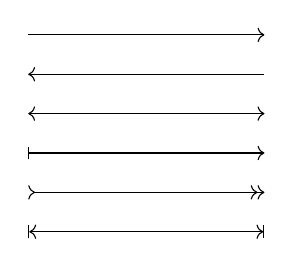
\begin{tikzpicture}
				\draw[->] (0,2.5) -- (3,2.5);
				\draw[<-] (0,2) -- (3,2);
				\draw[<->] (0,1.5) -- (3,1.5);
				\draw[|->] (0,1) -- (3,1);
				\draw[>->>] (0,0.5) -- (3,0.5);
				\draw[|<->|] (0,0) -- (3,0);
			\end{tikzpicture}
		\end{example}
	\item 连续绘制
	\begin{example}
		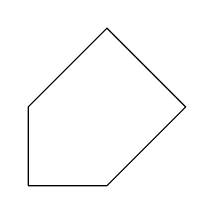
\begin{tikzpicture}
			\draw (0,0) -- (0,1) -- (1,2)
			 -- (2,1) -- (1,0) -- (0,0);
		\end{tikzpicture}
	\end{example}
	\item 直角折线
	\begin{example}
		\begin{tikzpicture}
			\draw (0,0) |- (1,1);
			\draw (1,0) -| (2,1);
		\end{tikzpicture}
	\end{example}
	\item 改变线宽
	\begin{example}
		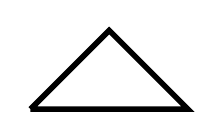
\begin{tikzpicture}[line width=
			2pt]
			\draw (0,0) -- (1,1) 
			 -- (2,0) -- (0,0);
		\end{tikzpicture}
	\end{example}
	\item 封闭缺口
	\begin{example}
		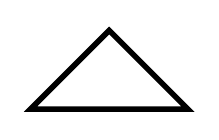
\begin{tikzpicture}[line width=
			2pt]
		\draw (0,0) -- (1,1) 
		-- (2,0) -- cycle;
		\end{tikzpicture}
	\end{example}
	\item 绘制矩形
	\begin{example}
	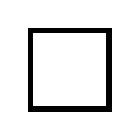
\begin{tikzpicture}[line width=
		2pt]
		\draw (0,0) rectangle (1,1);
	\end{tikzpicture}
	\end{example}
	\item 绘制网格
	\begin{example}
		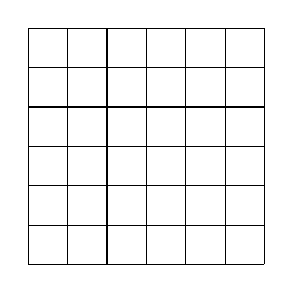
\begin{tikzpicture}
			% step指明网格间隔
			\draw[step=0.5](0,0) grid (3,3);
		\end{tikzpicture}
	\end{example}
\end{itemize}

\end{document}
